\documentclass[12pt, letterpaper]{article}

\usepackage{amsmath, enumerate, graphicx}
%\usepackage[showframe]{geometry}
\usepackage{layout}
\DeclareMathOperator*{\argmin}{argmin}
\DeclareMathOperator*{\argmax}{argmax}
\newcommand{\bv}[1]{\mathbf{#1}}

\title{CS 676\\ Problem Set 1a}

\author{Josh Wheeler, Yotam Barnoy}

\setlength{\voffset}{-0.75in}
\setlength{\headsep}{5pt}
\setlength{\hoffset}{-0.5in}
\setlength{\textwidth}{450pt}

\begin{document}%\layout

\maketitle

\setcounter{section}{1}

\section{Variational Inference on a Simple Network}
\subsection{Empirical Questions}
\begin{enumerate}[a.]
\item TODO
\item Mean field is a very crude approximation for the original distribution. We note that the KL divergence is very high ($0.829$), indicating that our approximate distribution is a bad choice.
\item Structured mean field inference is a far better approximation for our original distribution. The KL divergence is much lower than in the previous case ($0.002$), indicating the closeness of the approximation. Additionally, the values in the approximate marginal multinomial distribution are within roughly $0.01$ of the true distribution.

Mean field inference makes many independence assumptions missing from the original model. Structured mean field inference does this a lot less.
\end{enumerate}

\setcounter{section}{4}
\section{Blocked Gibbs}
\subsection{Derivation}
TODO

\section{Text Analysis with MCLDA}
\subsection{Empirical Questions}
\begin{enumerate}[1.]
    \item 
        We observe that all three graphs are very similar. No matter the random starting point, we still converge to a similar log likelihood for both the test and train data. 

        The shape of both the train and test curves is similar: we observe a generally increasing pattern approaching an asymptote. The two curves do differ in magnitude significantly though. The training data has much lower likelihood because it has more data, causing more probabilities to be multiplied together.

        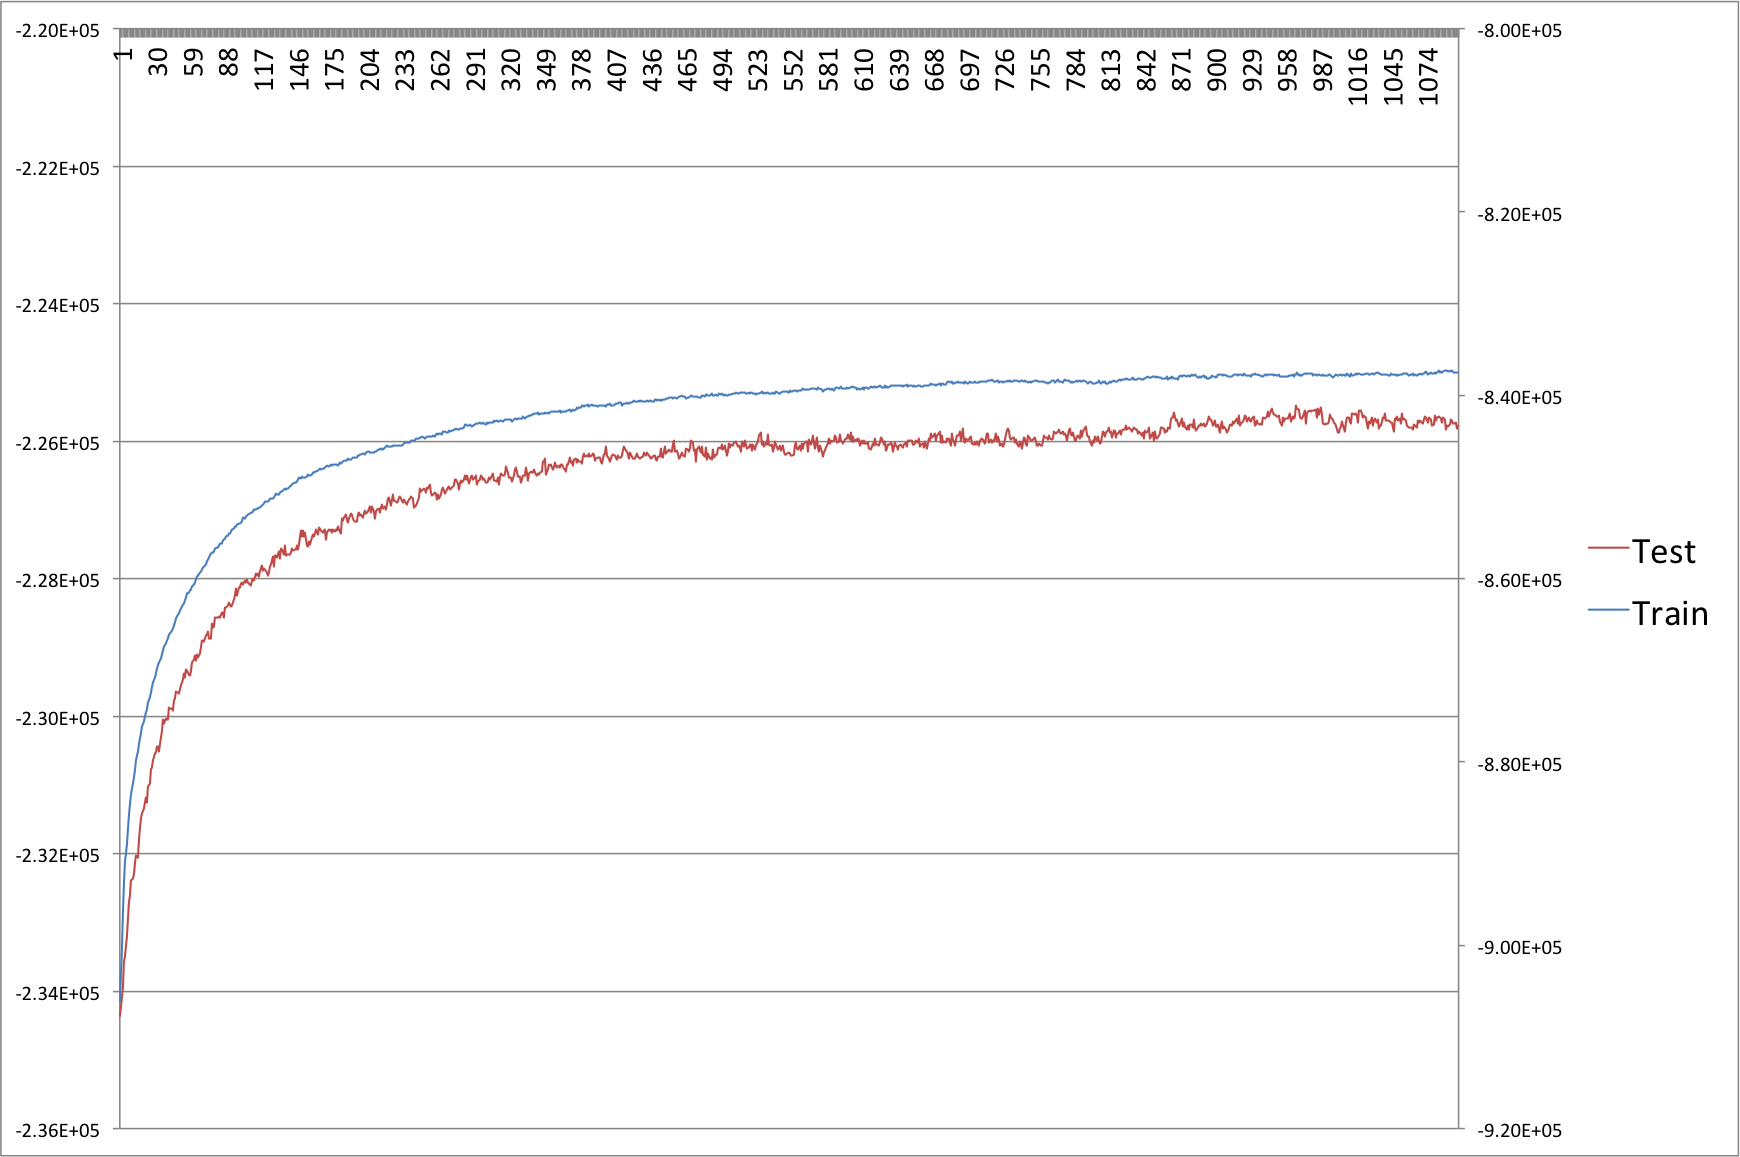
\includegraphics[scale=0.5]{ml_graph_1a}\\
        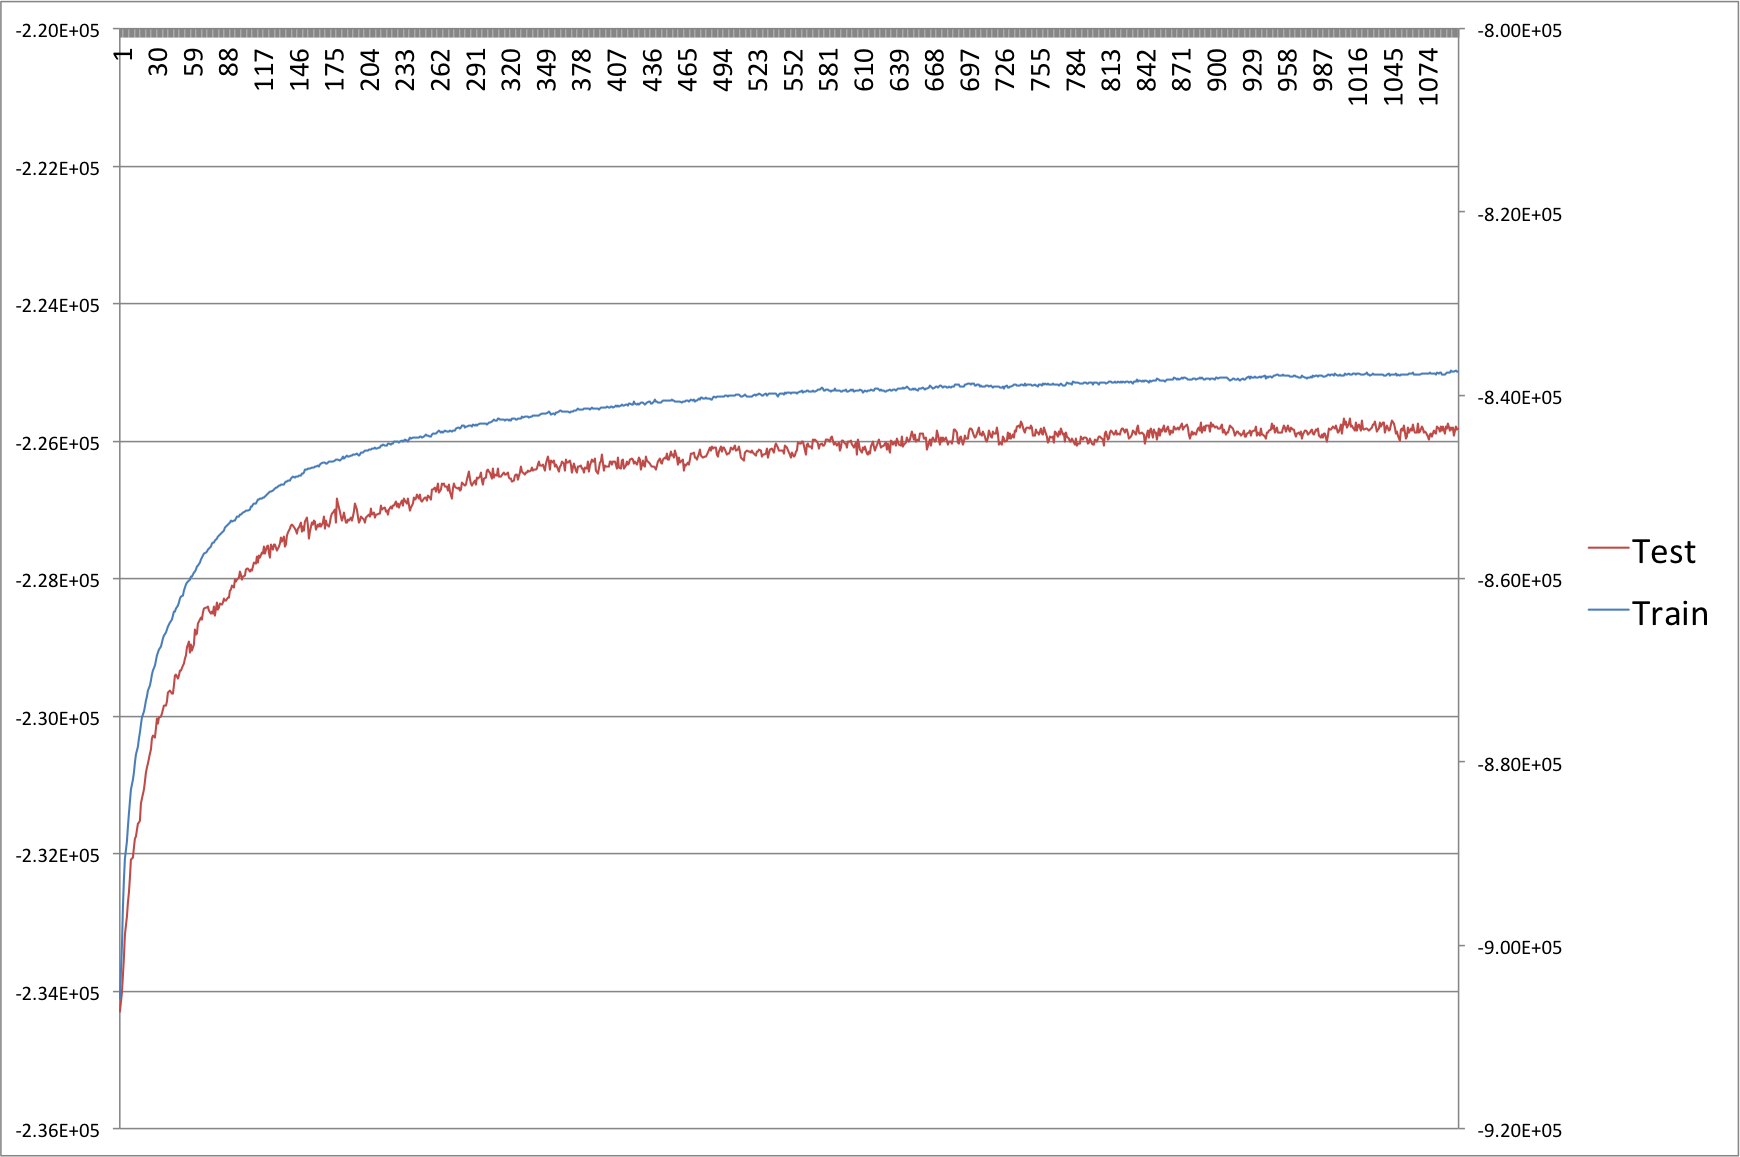
\includegraphics[scale=0.5]{ml_graph_1b}\\
        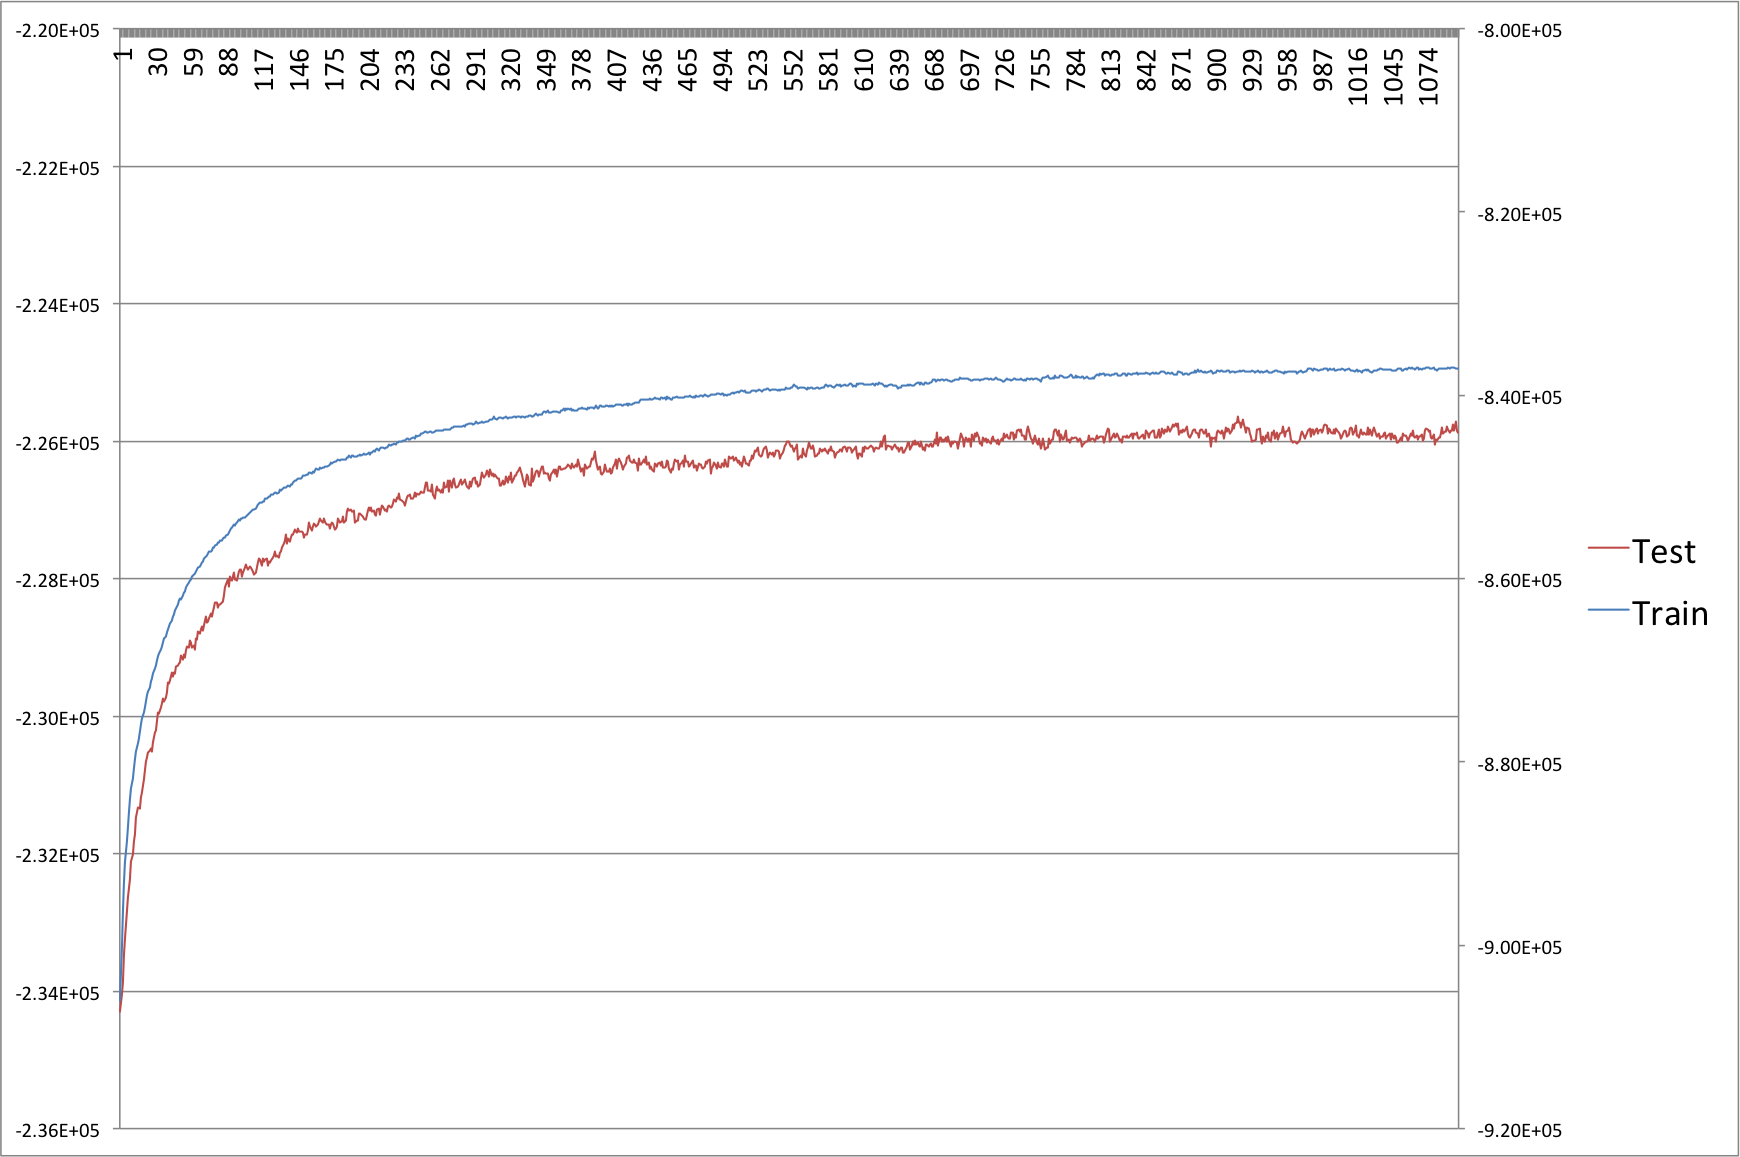
\includegraphics[scale=0.5]{ml_graph_1c}\\

    \item 
        The Blocked Gibbs sampler appears to converge much sooner than does the regular Gibbs sampler. We also noticed that the log-likelihood asymptote for Blocked Gibbs was lower than for the Gibbs sampler.

        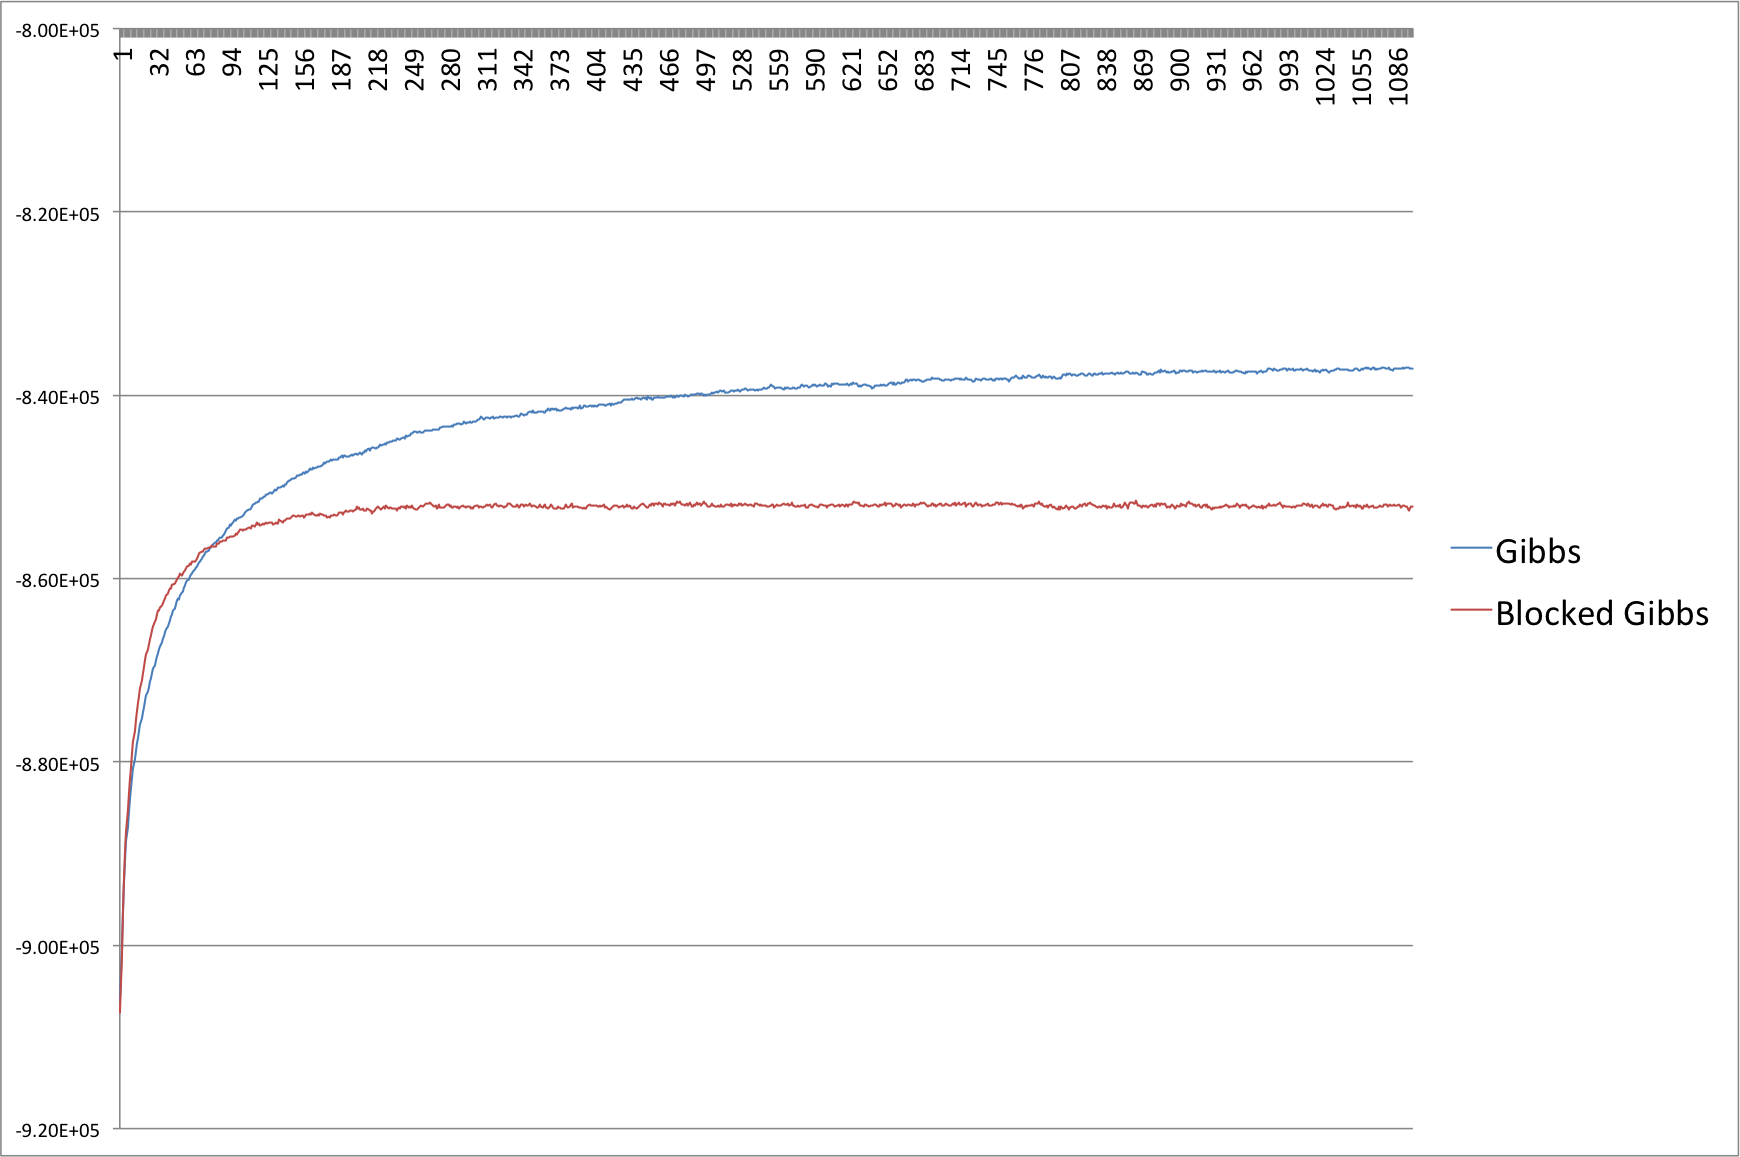
\includegraphics[scale=0.5]{ml_graph_2}\\

   \item
       While the Gibbs sampler is faster per iteration, ending its run in almost half the time, the Blocked Gibbs sampler still converges to a stable point much faster, making it more efficient overall.

       TODO: label graphs so it's obvious which is with time

        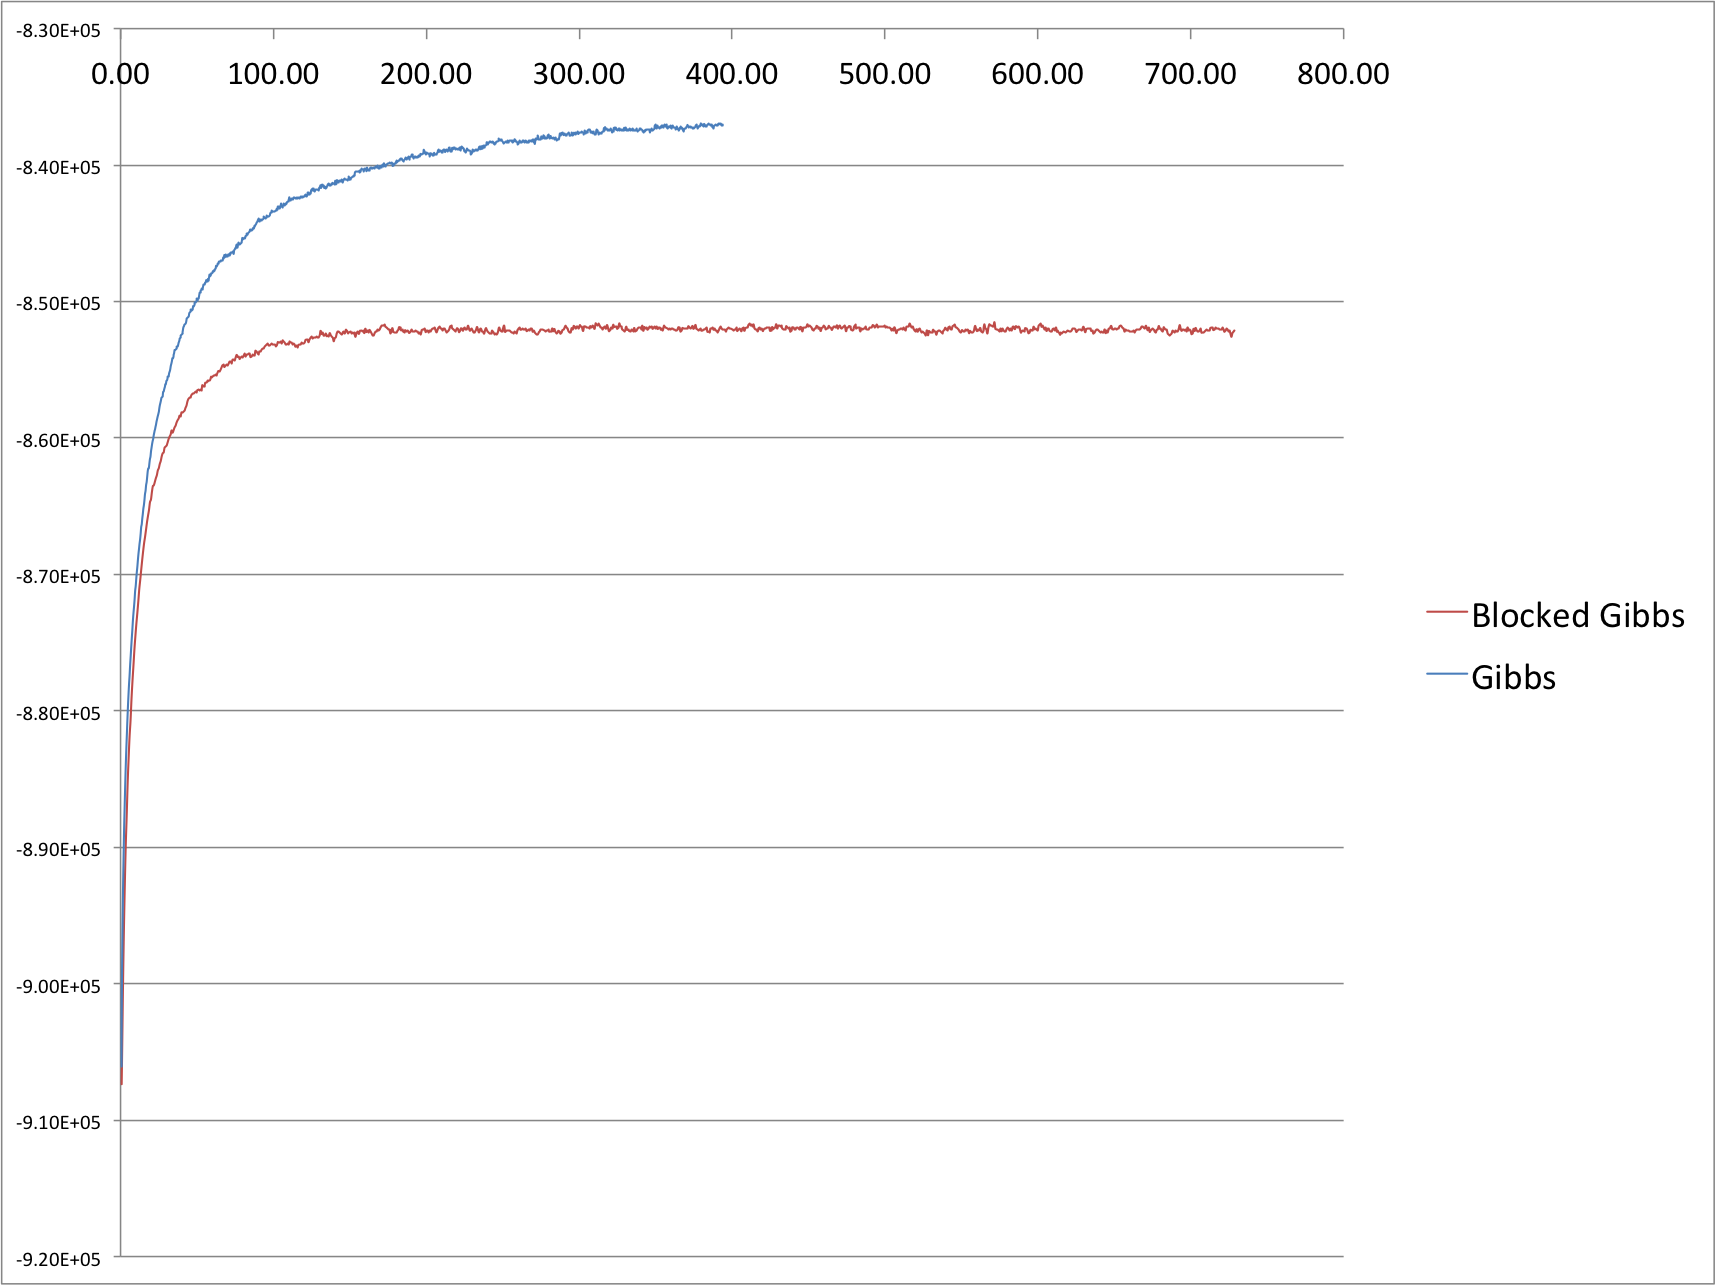
\includegraphics[scale=0.5]{ml_graph_3}\\

   \item 
       The test likelihood increases as the number of topics increases.

        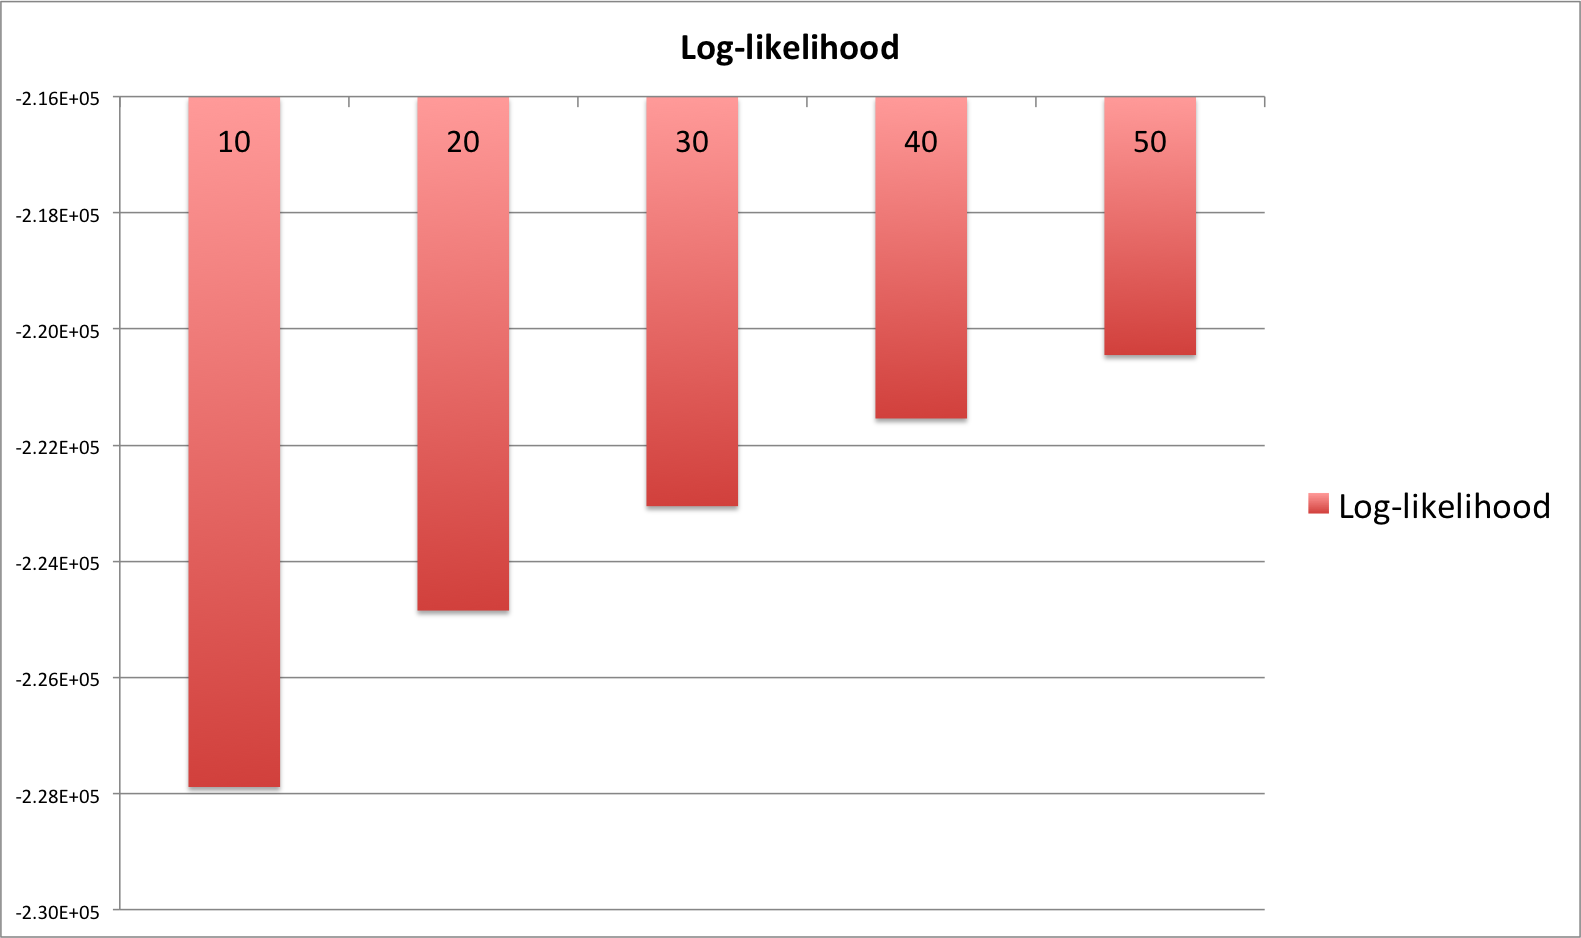
\includegraphics[scale=0.5]{ml_graph_4}\\

   \item
       The test likelihood increases as lambda increases.

        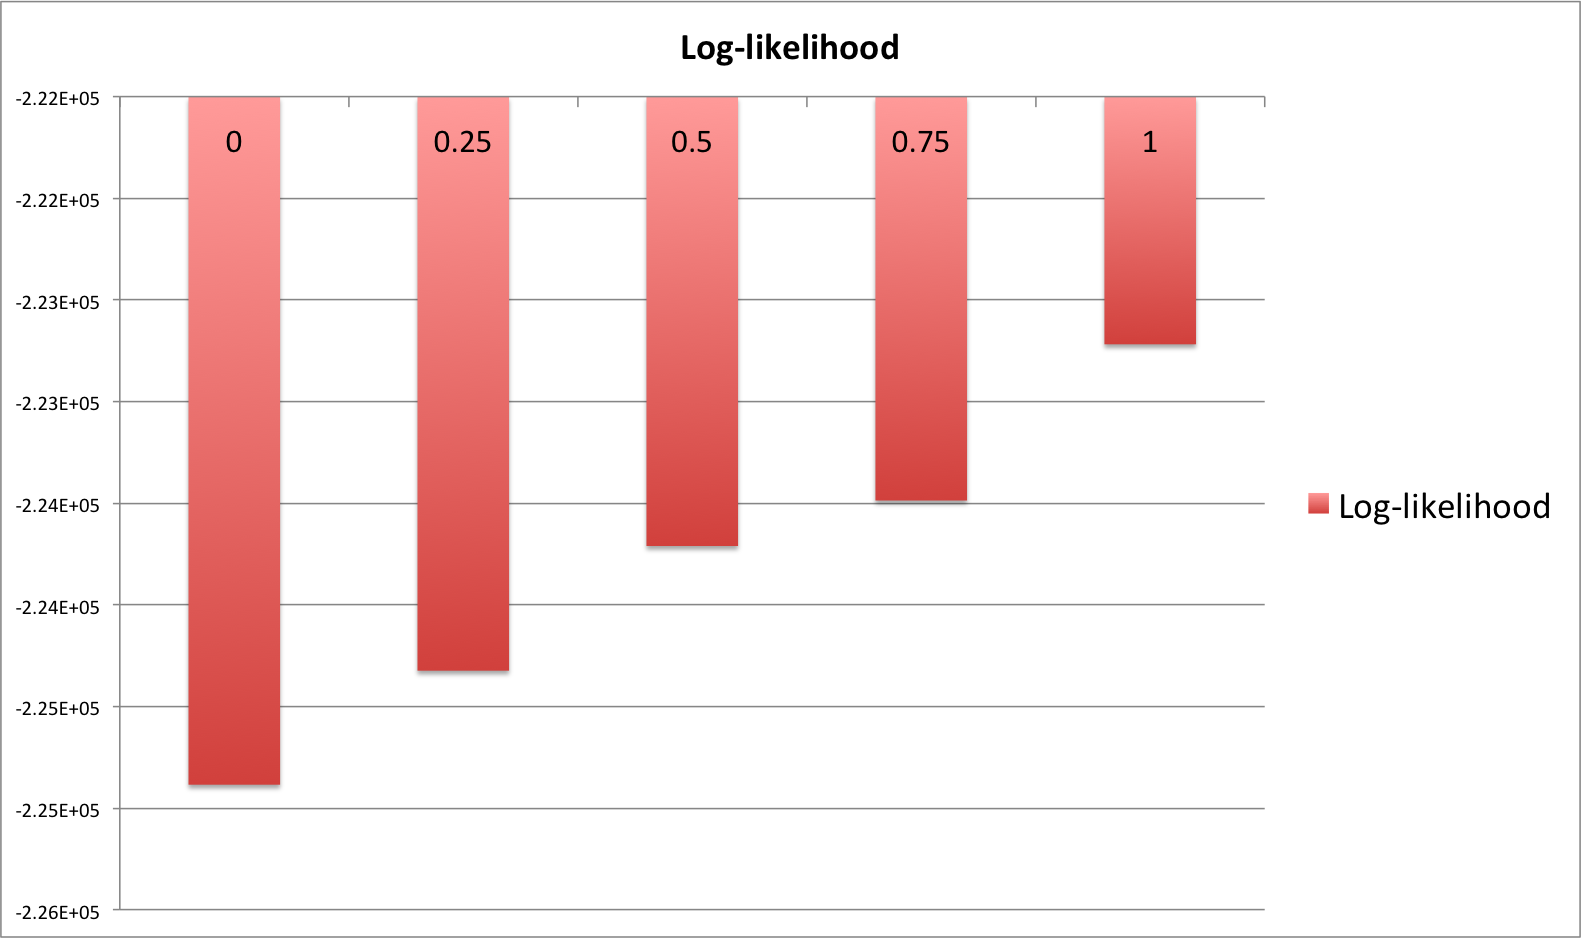
\includegraphics[scale=0.5]{ml_graph_5}\\

   \item
      \begin{enumerate}
          \item 
              We tried looking at 25 topics, 10 topics and 5 topics. At the 25 topic level, it was very hard to find any commonality between the corpora. The same is true for the 10 topic level. At the 5 topic level, words like method(s) could sometimes be found in common. However, in general, the global corpus tends to pick words that are... well, general. Words like `input', `model', `paper', that describe scholarship in general but with little specificity were common in the general corpus. On the other hand, the specific corpora picked up on specific topics of machine learning, often separating them neatly into different topics.
      \end{enumerate}


      

\end{enumerate}

\end{document}
